\documentclass[tikz,border=8pt]{standalone}

\usepackage{xcolor}
\definecolor{myblue}{HTML}{377EB8}
\definecolor{myred}{HTML}{E41A1C}
\definecolor{myviolet}{HTML}{984EA3}
\definecolor{mygray}{HTML}{666666}
\definecolor{mylightblue}{HTML}{BFD9F2}
\definecolor{mylightred}{HTML}{F7C0C1}
\definecolor{mylightviolet}{HTML}{DCC7EC}

\usepackage{tikz}
\usepackage{pgfplots}
\pgfplotsset{compat=1.18}

\usepackage{lmodern}
\SetSymbolFont{letters}{bold}{OML}{cmbr}{bx}{it}
\renewcommand{\familydefault}{\sfdefault}
\usepackage{sansmathfonts}

\begin{document}

% Dots are fixed effects (alpha).
% Thin black whiskers are 95% CIs for the fixed effects.
% Thick pale bars are approximate 95% between-person intervals:
% alpha +/- 1.96 * sqrt(tau^2_pp).

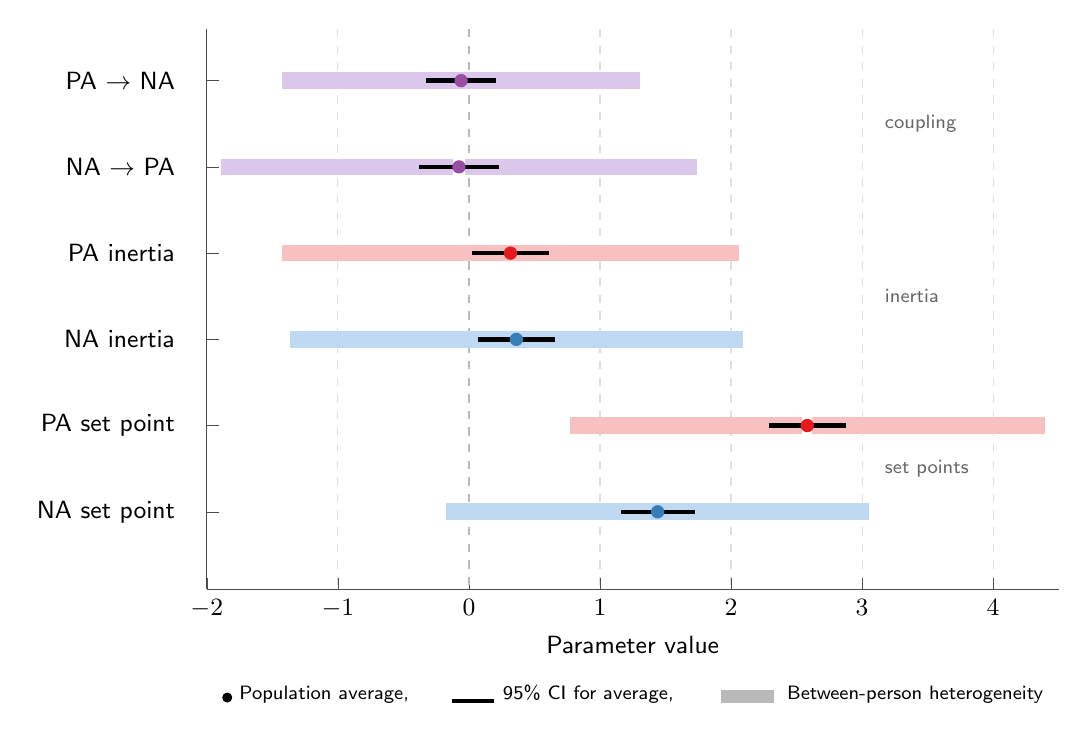
\begin{tikzpicture}
	\begin{axis}[
			width=12.4cm,
			height=8.7cm,
			xmin=-2, xmax=4.5,
			ymin=0.4, ymax=6.9,
			xlabel={Parameter value},
			xtick={-2,-1,0,1,2,3,4},
			ytick={1,2,3,4,5,6},
			yticklabels={,,,,,},
			tick label style={font=\small},
			label style={font=\small},
			axis x line*=bottom,
			axis y line*=left,
			axis line style={black!70},
			tick style={black!70},
			xmajorgrids,
			grid style={dashed,gray!25},
			y dir=reverse,
			clip=false,
			enlargelimits=false,
		]
				
		% zero reference
		\addplot[gray!55, dashed, line width=0.9pt, forget plot]
		coordinates {(0,0.4) (0,6.9)};
				
		% between-person heterogeneity intervals (outer bands)
		\addplot[only marks, mark=-, mark size=42pt, line width=6pt, color=mylightviolet]
		coordinates {(-0.5383,1) (-1.0073,2)};
		\addplot[only marks, mark=-, mark size=42pt, line width=6pt, color=mylightred]
		coordinates {(-0.5382,3) (1.6568,5)};
		\addplot[only marks, mark=-, mark size=42pt, line width=6pt, color=mylightblue]
		coordinates {(-0.4793,4) (0.7139,6)};
		\addplot[only marks, mark=-, mark size=42pt, line width=6pt, color=mylightviolet]
		coordinates {(0.4187,1) (0.8551,2)};
		\addplot[only marks, mark=-, mark size=42pt, line width=6pt, color=mylightred]
		coordinates {(1.1722,3) (3.5066,5)};
		\addplot[only marks, mark=-, mark size=42pt, line width=6pt, color=mylightblue]
		coordinates {(1.2027,4) (2.1665,6)};
				
		% fixed-effect 95% CIs (inner whiskers)
		\addplot[only marks, mark=-, mark size=11pt, line width=1.6pt, color=black, forget plot]
		coordinates {(-0.0963,1) (-0.1474,2)};
		\addplot[only marks, mark=-, mark size=11pt, line width=1.6pt, color=black, forget plot]
		coordinates {(0.2555,3) (2.5187,5)};
		\addplot[only marks, mark=-, mark size=11pt, line width=1.6pt, color=black, forget plot]
		coordinates {(0.3011,4) (1.3907,6)};
		\addplot[only marks, mark=-, mark size=11pt, line width=1.6pt, color=black, forget plot]
		coordinates {(-0.0233,1) (-0.0047,2)};
		\addplot[only marks, mark=-, mark size=11pt, line width=1.6pt, color=black, forget plot]
		coordinates {(0.3784,3) (2.6448,5)};
		\addplot[only marks, mark=-, mark size=11pt, line width=1.6pt, color=black, forget plot]
		coordinates {(0.4224,4) (1.4898,6)};
				
		% fixed-effect points
		\addplot[only marks, mark=*, mark size=2.2pt, color=myviolet]
		coordinates {(-0.0598,1) (-0.0761,2)};
		\addplot[only marks, mark=*, mark size=2.2pt, color=myred]
		coordinates {(0.3170,3) (2.5817,5)};
		\addplot[only marks, mark=*, mark size=2.2pt, color=myblue]
		coordinates {(0.3617,4) (1.4402,6)};
				
		% subtle group labels
		\node[anchor=west, font=\scriptsize, text=mygray] at (axis cs:3.1,1.5) {coupling};
		\node[anchor=west, font=\scriptsize, text=mygray] at (axis cs:3.1,3.5) {inertia};
		\node[anchor=west, font=\scriptsize, text=mygray] at (axis cs:3.1,5.5) {set points};
				
		% parameter labels outside the plotting region
		\node[anchor=east, font=\small] at ([xshift=-8pt]axis cs:-2,1) {PA $\rightarrow$ NA};
		\node[anchor=east, font=\small] at ([xshift=-8pt]axis cs:-2,2) {NA $\rightarrow$ PA};
		\node[anchor=east, font=\small] at ([xshift=-8pt]axis cs:-2,3) {PA inertia};
		\node[anchor=east, font=\small] at ([xshift=-8pt]axis cs:-2,4) {NA inertia};
		\node[anchor=east, font=\small] at ([xshift=-8pt]axis cs:-2,5) {PA set point};
		\node[anchor=east, font=\small] at ([xshift=-8pt]axis cs:-2,6) {NA set point};
		
		% centered one-line legend below the plot
		\node[
			anchor=north,
			font=\scriptsize,
			inner sep=0pt
			] at ([yshift=-34pt]rel axis cs:0.5,0) {%
					\begin{tabular}{@{}c@{\hspace{0.35em}}l@{\qquad}c@{\hspace{0.35em}}l@{\qquad}c@{\hspace{0.35em}}l@{}}
						\raisebox{-0.35ex}{\tikz \filldraw[black] (0,0) circle (1.6pt);}             &   
						Population average,                                                          &   
						\raisebox{-0.35ex}{\tikz \draw[black,line width=1.3pt] (0,0) -- (0.32,0);}   &   
						95\% CI for average,                                                         &   
						\raisebox{-0.35ex}{\tikz \draw[gray!55,line width=4.5pt] (0,0) -- (0.40,0);} &   
						Between-person heterogeneity
					\end{tabular}%
					};
							
					\end{axis}
					\end{tikzpicture}
					
\end{document}
